

\section{Abstract}
The Ising model in two dimensions was examined to understand phase transitions for a ferromagnetic canonical system. Without the application of an external magnetic field the Ising model is in it's simplest form.\\


I find that the Monte Carlo simulation and analytical solutions coincide with very small error ($O(10^{-3})$) for number of trials above $10^5$ with T=1 and T=2.4. The exception is the average magnetization per spin and susceptibility per spin for T=1, which seems to have unstable solutions  for number of trials above $10^3$





\section{Introduction}
In this project I will study the Ising model in two dimensions. This model is used to simulate phase transitions. When reaching the critical temperature $T_c$ the model gives a phase transition from a system with finite magnetic moment, to a phase with zero magnetization. At the critical temperature we need to examine the system closely to understand how particles interact, since we can have large fluctuations in this transition phase.\\



The model is binary, and in our case we take advantage of that with the objects at each lattice having the option of being a spin up or spin down. These states characterizes the microstates of a substance. \cite{spin}\\




The one- and two- dimensional systems have analytical solutions for various expectation values. Ernst Ising solved the one-dimensional system in 1925. The two-dimensional system allows for phase transitions and was solved analytically by Lars Onsager in 1944 \cite{ising}.  We will look at the simplest two- dimensional case, where we do not allow an external magnetic field. In this case the energy is:


\begin{equation}
E = -J\sum_{<kl>}^Ns_ks_l
\end{equation}

, where J is the coupling constant expressing the strength of the interaction between neigboring spins. $<kl>$ indicates that we sum over the nearest neigbors only, e.g. that only neighboring spins interact with each other. N is the total number of spins. We will assume ferromagnetic ordering, 
$J > 0$, which implies a strong interaction between the electrons, hence a strong ordering. $s_k$ and $s_l$ are neighboring spins each represented with a value of $\pm 1$.\\




To model the phase transitions I will use Monte Carlo simulations, specifically the Metropolis algorithm with periodic boundary conditions. Periodic boundary conditions means that at the end of the lattice, we start over from the start of the lattice, e.g. the first and last lattice positions are neighbors.\\





\section{Methods}
\subsubsection{Analytical solutions}
The derivation is based on the lecture note on statistics for the ising model \cite{isingstat}\\



The Ising model is a typical canonical ensemble. The system allows for heat interaction, whilst holding fixed the volume, temperature and number of particles. The partition function is given by:

\begin{equation}
Z = \sum_ie^{-\beta E_i} 
\end{equation}

, where $\beta = 1/kT$, where k = Boltzmann's constant and T = temperature, $E_i$ is the energy for each microstate.\\


The Boltzmann probability distribution is given as $P_i$:

\begin{equation}
P_i(\beta) = \frac{e^{-\beta E_i}}{Z} 
\end{equation}\\


The mean energy is given as:
\begin{equation}
<E> = \sum_i^ME_iP_i(\beta) = \frac{1}{Z}\sum_i^ME_ie^{-\beta E_i}
\end{equation}\\


And the corresponding specific heat $C_v=\frac{1}{kT^2}$, k and T again being Boltzmann's constant and temperature, is represented by the variance:

\begin{equation}
\sigma^2 = <E^2> - <E>^2 = \frac{1}{Z}\sum_i^ME_i^2e^{-\beta E_i}-(\frac{1}{Z}\sum_i^ME_ie^{-\beta E_i})^2
\end{equation}\\

\begin{equation}
<|M|> = \sum_i^M|M_i|P_i(\beta)
\end{equation}


\begin{equation}
\chi = \frac{<M^2> - <M>^2}{kT^2}
\end{equation}

,where k is Boltzmann's constant and T is temperature

For the 2 by 2 lattice with only neighbors interacting, with either positive or negative spin, I find the same values as found on page 9 of \cite{isingstat}:


\FloatBarrier
\begin{table}

\begin{tabular}{lrrrr}
\toprule
Number spins up &  Degeneracy &  Energy (Ei) &  Magnetization (Mi) \\
\midrule
4 &      1 &      -8J &        4 \\
3 &      4 &      0 &        2 \\
2 &      4 &      0 &        0 \\
2 &      2 &      8J &        0 \\
1 &      4 &      0 &        -2 \\
0 &      1 &      -8J &        -4 \\
\bottomrule

\end{tabular}

\caption{List of configurations with energies and magnetic moment}
\label{tab:Configurations_energy_magnetic}
\end{table}
\FloatBarrier


\subsubsection{Analytical values}
By using table ~\ref{tab:Configurations_energy_magnetic} and inserting values into the theoretical expressions for the partition function, expected energy, specific heat, mean expected absolute value of magnetic moment and susceptibility.\\


Analytical values was calculated to be:\\

\begin{equation}
Z = 12+4cosh(8\beta J)
\end{equation}

\begin{equation}
<E> = \frac{-8Jsinh(8\beta J)}{cosh(8\beta J + 3}
\end{equation}

\begin{equation}
<|M|> = \frac{2e^{8\beta J}+4}{cosh(8\beta J)+3}
\end{equation}

\begin{equation}
\chi = \frac{8(e^{8\beta J}+1)}{(cosh(8\beta J)+3)kT}
\end{equation}

\subsection{Metropolis algorithm}
The metropolis algorithm is a smart method for evaluating a model for a system with not fully disclosed probabilities since it only requires an approximation for the initial probability. Even if we don't know the point density function of the system, we can use a function which is proportional to the original function. In our case we could estimate the exact probability function, but it's very time consuming. Luckily for us we don't need to use the partition function, because the Metropolis-Hastings algorithm only considers the ratio between probabilities. Instead we use rejection sampling.\\




First we calculate the energy of the current state. Then we change the initial configuration by flipping only one spin. Then we compute the energy for this trial state. Then we calculate the energy in the previous step and the current step.  If $\Delta E$, the change in energy, is negative, we accept the new configuration. This means that the energy is lowered, and hopefully we are moving towards the equilibrium state. We also must consider accepting a move if it increases the energy. This is done by rejection sampling. Rejection sampling is done by choosing a random number and comparing it with the weight 
$e^{-\beta \Delta E}$, where beta = 1/kT and $\Delta E$ is the change of energy. If the random number is smaller than the weight, we accept the new configuration, otherwise we keep the old configuration. The next step is to update various expectation values. These steps are then repeated to get a sufficiently good representation of states. Each time we sweep through the lattice, constitutes a Monte Carlo Cycle. \cite{lecturenote} page 435 (Ch. 13.5)\\





\newpage
\section{Implementation}
For all programs, see:\\
$\href{https://github.com/larsjbro/FYS4150/tree/master/project_4/source}{https://github.com/larsjbro/FYS4150/tree/master/project_4/source}$


\subsection{Metroplis algorithm}
The metropolis algorithm is used to accept or reject a move, implemented with the following code:

\begin{lstlisting}
def metropolis(E, M, w, size, spin_matrix):
    # Metropolis
    # Loop over all spins, pick a random spin each time
    for s in xrange(size**2):
        x = int(numpy.random.random() * size)
        y = int(numpy.random.random() * size)
        deltaE = 2 * spin_matrix[x, y] * (spin_matrix[periodic(x, size, -1), y]
                                          + spin_matrix[periodic(x, size, 1), y]
                                          + spin_matrix[x, periodic(y, size, -1)]
                                          + spin_matrix[x, periodic(y, size, 1)])

        accept = numpy.random.random() <= w[deltaE + 8]
        if accept:
            spin_matrix[x, y] *= -1
            M += 2 * spin_matrix[x, y]
            E += deltaE
    return E, M
\end{lstlisting}

Since we are only calculating energy between two neighboring spins, the change in energy is simplified as $2*spin\_matrix$ which is also shown in equation 13.6 in \cite{isingstat}. How we accept a move was discussed in the method for the metropolis algorithm above, and implemented as such in the code above. 


\subsection{Calculating the critical parameters with Monte Carlo}
Added spin matrix to the existing algorithm for Monte Carlo given on the course material site. The given function from the course, is called monteCarlo. Here I calculate the values for energy, specific heat, magnetization and susceptibility. These can then be compared to the analytical results, which is done in the results section.

\begin{lstlisting}
def compute_monte_carlo(temperature, size, trial_sizes, spin_matrix='ordered'):
    data = []
    for trials in trial_sizes:
        print trials
        t0 = timer()
        data.append(monteCarlo(temperature, size, trials, spin_matrix=spin_matrix))
        print 'elapsed time: {} seconds'.format(timer() - t0)

    data = np.array(data)
    names = ['Average Energy per spin $E/N$',
             'Specific Heat per spin $C_V/N$',
             'Average Magnetization per spin $M/N$',
             'Susceptibility per spin $var(M)/N$',
             'Average |Magnetization| per spin $|M|/N$',
             'Variance of |Magnetization| per spin $var(|M|)/N$',
             'Number of accepted configurations']
    return data, names
\end{lstlisting}


\subsection{Finding the most likely state}
Below is the code used to find the number of Monte Carlo cycles to reach the equlibrium state for a lattice of size 20 times 20, for trials up to $10^5$

\begin{lstlisting}
def task_c(temperatures=(1,)):
    trial_sizes = [10, 30, 100, 300, 1000, 3000, 10000, 30000, 100000] # 10**np.arange(1, 5)
    for temperature in temperatures:
        print temperature
        size = 20
        for spin_matrix in ['ordered', 'random']:
            data, names = compute_monte_carlo(temperature, size, trial_sizes, spin_matrix)

            plt.figure()
            plot_mean_energy_and_magnetization(trial_sizes, data, names, temperature, spin_matrix)
            plt.savefig('task_c_T{}_size{}_{}.png'.format(temperature, 20, spin_matrix))

            plt.figure()
            plot_total_number_of_accepted_configs(trial_sizes, data, names, temperature, spin_matrix)
            plt.savefig('task_c_accepted_T{}_size{}_{}.png'.format(temperature, 20, spin_matrix))
\end{lstlisting}



%*Code/Implementations/test: Readability of code, implementation, testing and discussion of benchmarks. Total number of possible points 20*

 

\section{Results}
%*Analysis: of results and the effectiveness of their selection and presentation. Are the results well understood and discussed? Total number of possible points: 20*

\subsection{Agreement between analytical and numerical simulations and the equilibrium state}

From the figures 1 and 2 below I can see that temperature T=1 is the hard problem, when the magnetization has unstable solutions for many Monte Carlo cycles. For T=2.4 solutions are acceptable to order $10^{-3}$ when we approach $10^5$ trials. This is also when we reach an approximate equilibrium state for T=2.4. For T=1 the equilibrium state is trapped from the beginning and was never able to change state due to the temperature being too low to access other states. This can be seen in figure 3 and 4.

\FloatBarrier
\begin{figure}[!ht]
\centering
\FloatBarrier
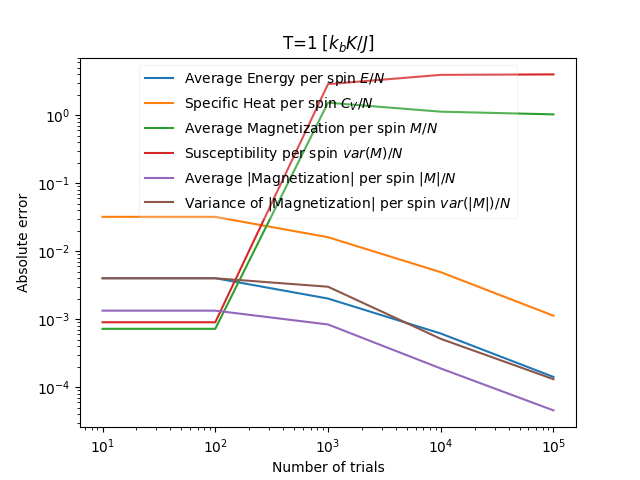
\includegraphics[width=0.70\textwidth]{task_b_abserr_T1_size2.png}

\caption{Absolute error between theoretical and simulated expected values for T=1}
\label{fig:Earth_orbit_sun_Forward_Euler_k_4}
\end{figure}
\FloatBarrier


\FloatBarrier
\begin{figure}[!ht]
\centering
\FloatBarrier
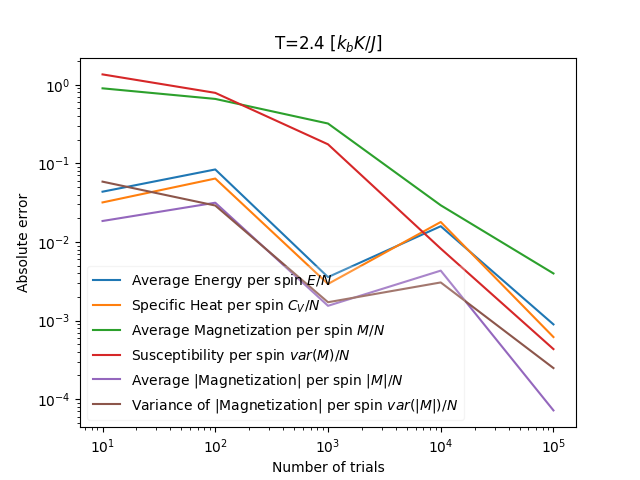
\includegraphics[width=0.70\textwidth]{task_b_abserr_T2_4_size2.png}

\caption{Absolute error between theoretical and simulated expected values for T=2.4}
\label{fig:Earth_orbit_sun_Forward_Euler_k_2}
\end{figure}
\FloatBarrier



\FloatBarrier
\begin{figure}[!ht]
\centering
\FloatBarrier
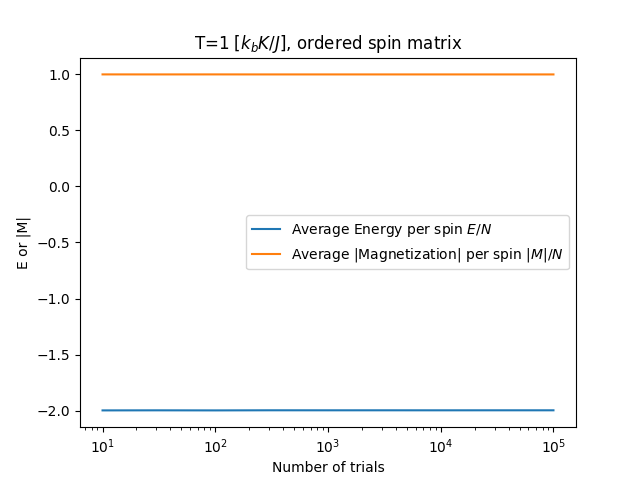
\includegraphics[width=0.70\textwidth]{task_c_T1_size20_ordered.png}

\caption{Approaching equlibrium state for T=1}
\label{fig:Earth_orbit_sun_Forward_Euler_k_2}
\end{figure}
\FloatBarrier


\FloatBarrier
\begin{figure}[!ht]
\centering
\FloatBarrier
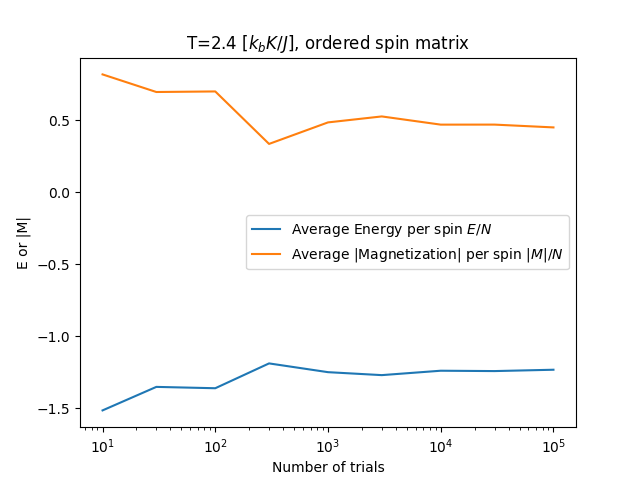
\includegraphics[width=0.70\textwidth]{task_c_T2_4_size20_ordered.png}

\caption{Approaching equlibrium state for T=2.4}
\label{fig:Earth_orbit_sun_Forward_Euler_k_2}
\end{figure}
\FloatBarrier

\subsection{Accepted configurations as a function of temperature}
From figure 5 and 6 below I see that accepted configurations go up with the temperature, meaning that more states are accessible for higher temperatures.


\FloatBarrier
\begin{figure}[!ht]
\centering
\FloatBarrier
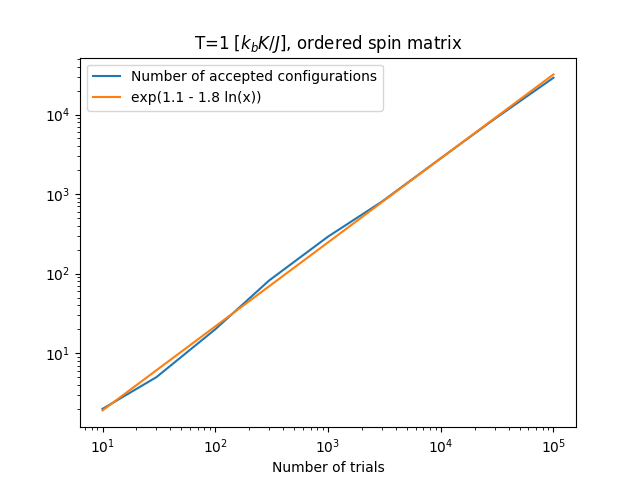
\includegraphics[width=0.70\textwidth]{task_c_accepted_T1_size20_ordered.png}

\caption{Accepted configurations as function of Monte Carlo cycles for T=1}
\label{fig:Earth_orbit_sun_Forward_Euler_k_2}
\end{figure}
\FloatBarrier



\FloatBarrier
\begin{figure}[!ht]
\centering
\FloatBarrier
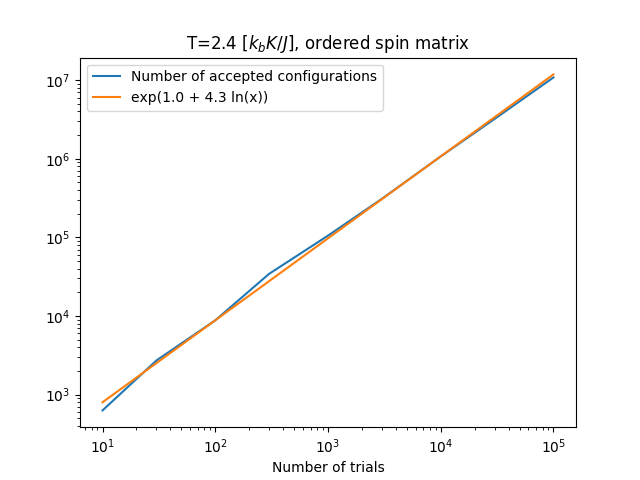
\includegraphics[width=0.70\textwidth]{task_c_accepted_T2_4_size20_ordered.png}

\caption{Accepted configurations as function of Monte Carlo cycles for T=2.4}
\label{fig:Earth_orbit_sun_Forward_Euler_k_2}
\end{figure}
\FloatBarrier


\subsection{Probability distribution}
I see from figure 7 and 8 that the probability for being in an energy state is more correlated in the lower temperatures. The variance of the distribution is very small, which is also reflected in the probability distribution.

\FloatBarrier
\begin{figure}[!ht]
\centering
\FloatBarrier
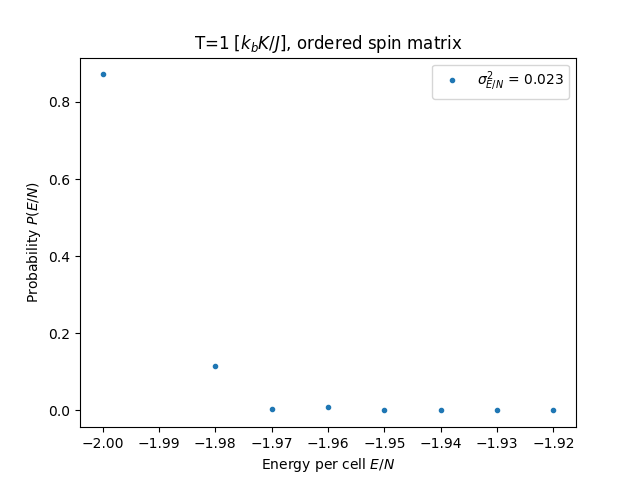
\includegraphics[width=0.70\textwidth]{task_d_probability_T1_size20_ordered.png}

\caption{Probability for being in different energy states for T=1}
\label{fig:Earth_orbit_sun_Forward_Euler_k_2}
\end{figure}
\FloatBarrier


\FloatBarrier
\begin{figure}[!ht]
\centering
\FloatBarrier
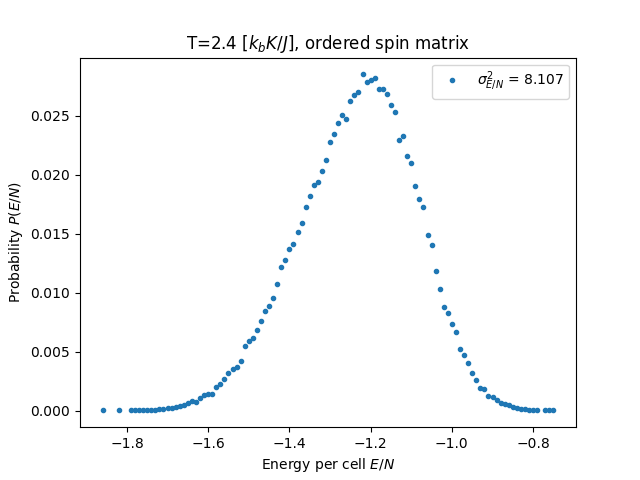
\includegraphics[width=0.70\textwidth]{task_d_probability_T2_4_size20_ordered.png}

\caption{Probability for being in different energy states for T=2.4}
\label{fig:Earth_orbit_sun_Forward_Euler_k_2}
\end{figure}
\FloatBarrier




\section{Conclusion}
It takes a long time to run Monte Carlo cycles. I found that accepted configurations increase with temperature, and that the numerical expression had some issues for the magnetization for low temperatures and many trials. 

For $T<T_c$ the probability distribution is very sharp, meaning it's hard to get out of an energy state. 


%*Conclusions, discussions and critical comments: on what was learned about the method used and on the results obtained. Possible directions and future improvements? Total number of possible points: 10*




\begin{thebibliography}{99}
\bibitem{heisenberg} W. Heisenberg, Zeits. f. Physik {\bf 77}, 1 (1932).
\bibitem{miller2006} G.~A.~Miller, A.~K.~Opper, and E.~J.~Stephenson, Annu.~Rev.~Nucl.~Sci.~{\bf 56}, 253 (2006).
\bibitem{ekstrom2015} A.~Ekstr\"om, G.~R.~Jansen, K.~A.~Wendt, G.~Hagen, T.~Papenbrock, B.~D.~Carlsson, C.~Forssen, M.~Hjorth-Jensen, P.~Navratil, and W.~Nazarewicz, Phys.~Rev.~C {\bf 91}, 051301(R) (2015).
\bibitem{brown1977} B. A. Brown, A. Arima and J. B. McGrory, Nucl. Phys. {\bf A277}, 77 (1977) and references therein.
\bibitem{ising} $\href{https://en.wikipedia.org/wiki/Ising\_model}{https://en.wikipedia.org/wiki/Ising\_model}$
\bibitem{lecturenote}$\href{https://github.com/CompPhysics/ComputationalPhysics/blob/gh-pages/doc/Lectures/lectures2015.pdf}{https://github.com/CompPhysics/ComputationalPhysics/blob/gh-pages/doc/Lectures/lectures2015.pdf}$, November 19 2017\\
\bibitem{spin}$\href{https://en.wikipedia.org/wiki/Spin-\%C2\%BD}{https://en.wikipedia.org/wiki/Spin-\%C2\%BD}$\\
\bibitem{isingstat}$\href{http://compphysics.github.io/ComputationalPhysics/doc/pub/statphys/pdf/statphys-print.pdf}{http://compphysics.github.io/ComputationalPhysics/doc/pub/statphys/pdf/statphys-print.pdf}$
\end{thebibliography}



%\FloatBarrier
%\begin{figure}[!ht]
%\centering
%\FloatBarrier
%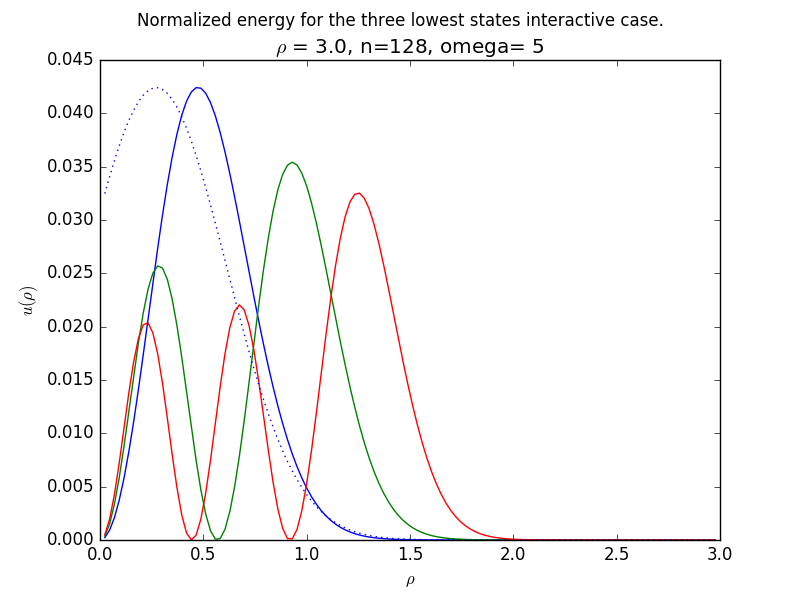
\includegraphics[width=0.45\textwidth]{eigenvector_rho29n128omega500.png}
%
%\caption{Normalized energy for the three lowest eigenvalues for repulsive Coulomb interaction with n=128 and $\omega_r$=5}
%\label{fig:Eigenvalue_states_n_320_omega_500}
%\end{figure}
%\FloatBarrier


